\part{Experiments and Validation}

In this section we present three test cases, Alexandrov Problem, Turbofan Problem and Viennet1, on which our system has been applied, and the experimental results we obtained. In each test cases, the MAS consistently converges towards the best (or one of the best) solution.

\begin{figure}
\centering
	\subfloat[mathematical formulation.]{\begin{minipage}{0.4\textwidth}%
		$\begin{array}{c}
			a_1 = (l_1 - a_2)/2 \\
			a_2 = (l_2 - a_1)/2 \\
			min \; \frac{1}{2}(a_1^2 + 10a_2^2 + 5(s-3)^2) \\
			subject \; to \\
			s + l_1 \leq 1 \\
			-s + l_2 \leq -2
		\end{array}$
		\label{alexandrov:math}
	\end{minipage}}\hfill%for spacing
	\subfloat[corresponding agent graph.]{\begin{minipage}{0.5\textwidth}%
		\centering
		\includegraphics[width=\textwidth]{testcases-Alexandrov}%screen_Alexandrov}%}
		\label{alexandrov:graph}
	\end{minipage}}
	\caption{Alexandrov problem}
	\label{alexandrov}
	\vspace{-20pt}
\end{figure}

\subsection{Alexandrov Problem}

\begin{figure}[t]
\centering

  \subfloat{\begin{minipage}{0.4\textwidth}%
		\centering
		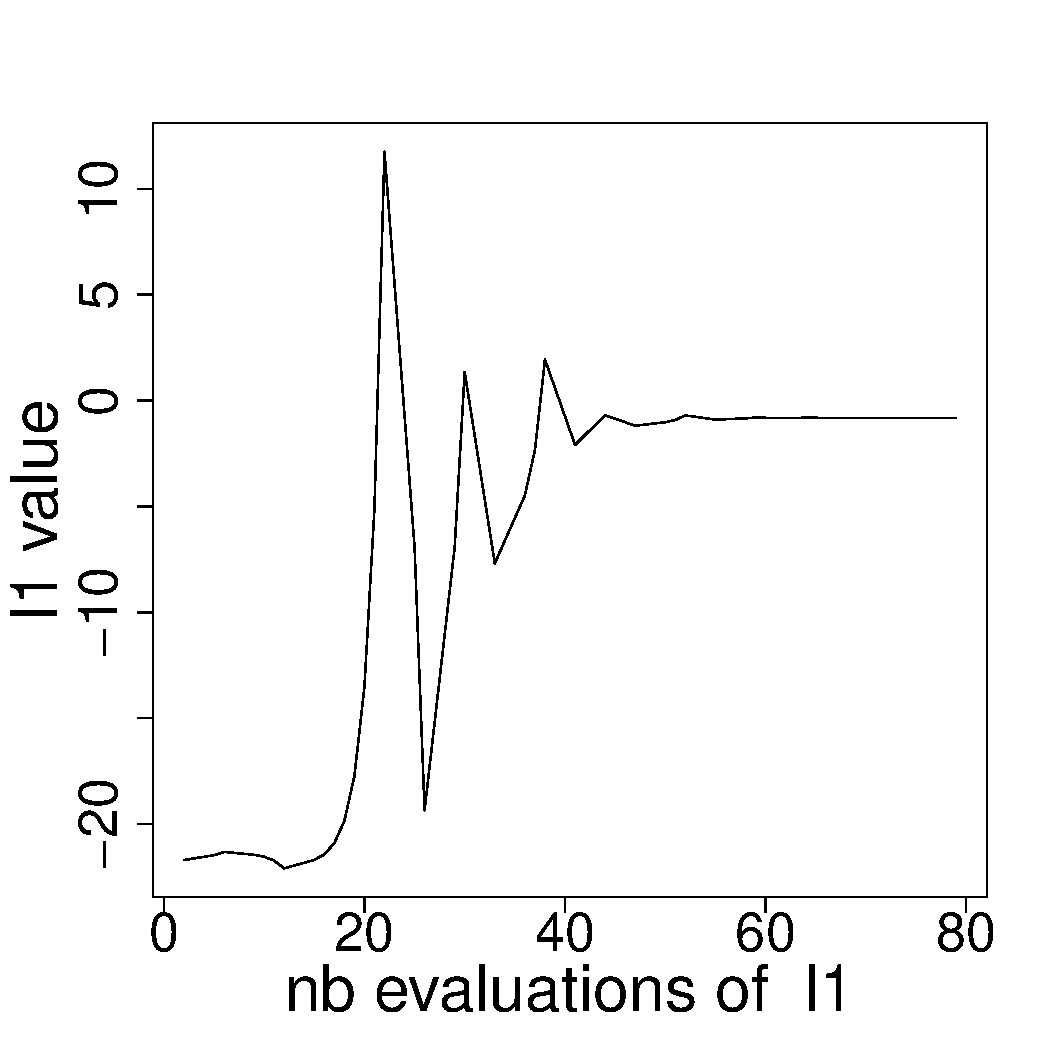
\includegraphics[width=\textwidth]{./R_figs/generated/l1_one_run}
		\vspace{-20pt}
		\label{alexandrov_res_one:l1}
	\end{minipage}}%
	\subfloat{\begin{minipage}{0.4\textwidth}%
		\centering
		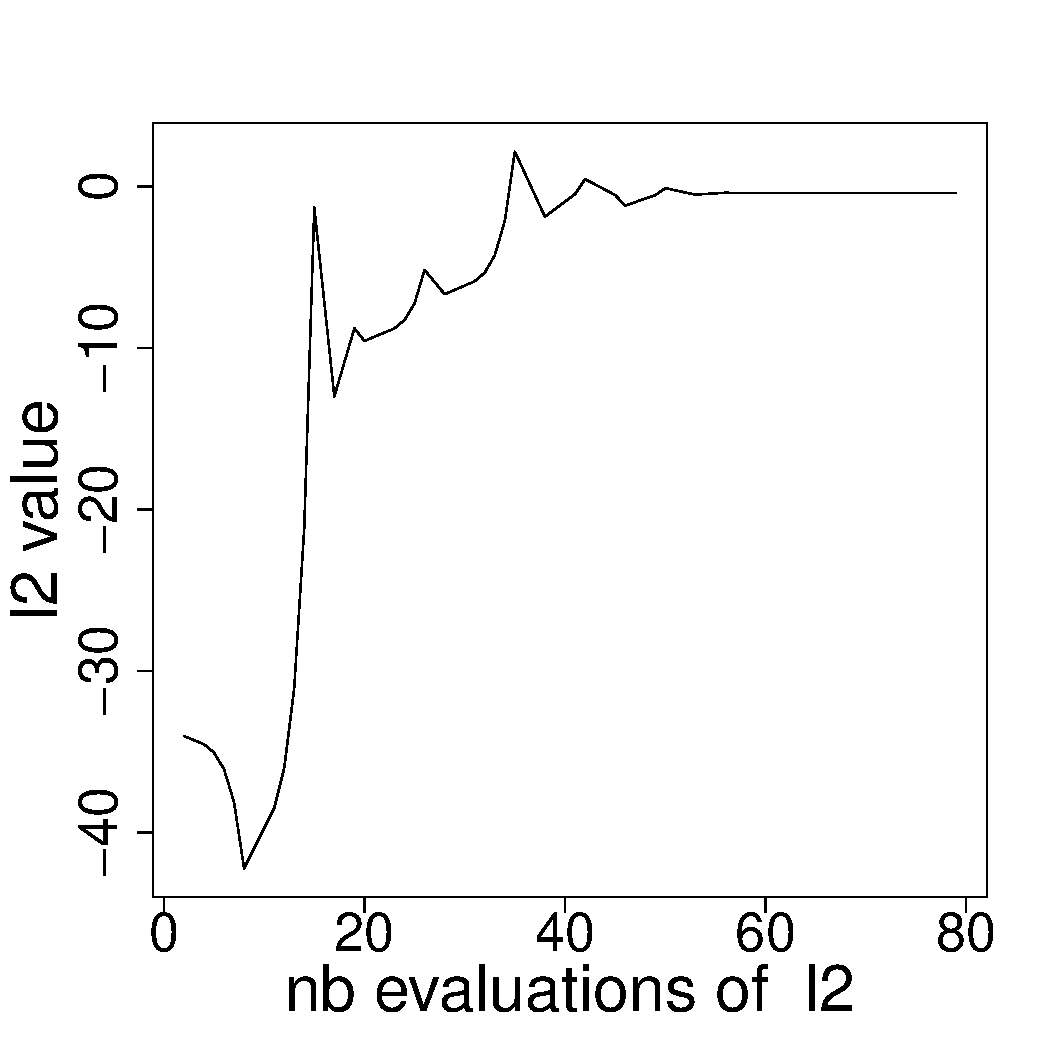
\includegraphics[width=\textwidth]{./R_figs/generated/l2_one_run}
		\vspace{-20pt}
		\label{alexandrov_res_one:l2}
	\end{minipage}}
	\vspace{-20pt}
	\\
	\subfloat{\begin{minipage}{0.4\textwidth}%
		\centering
		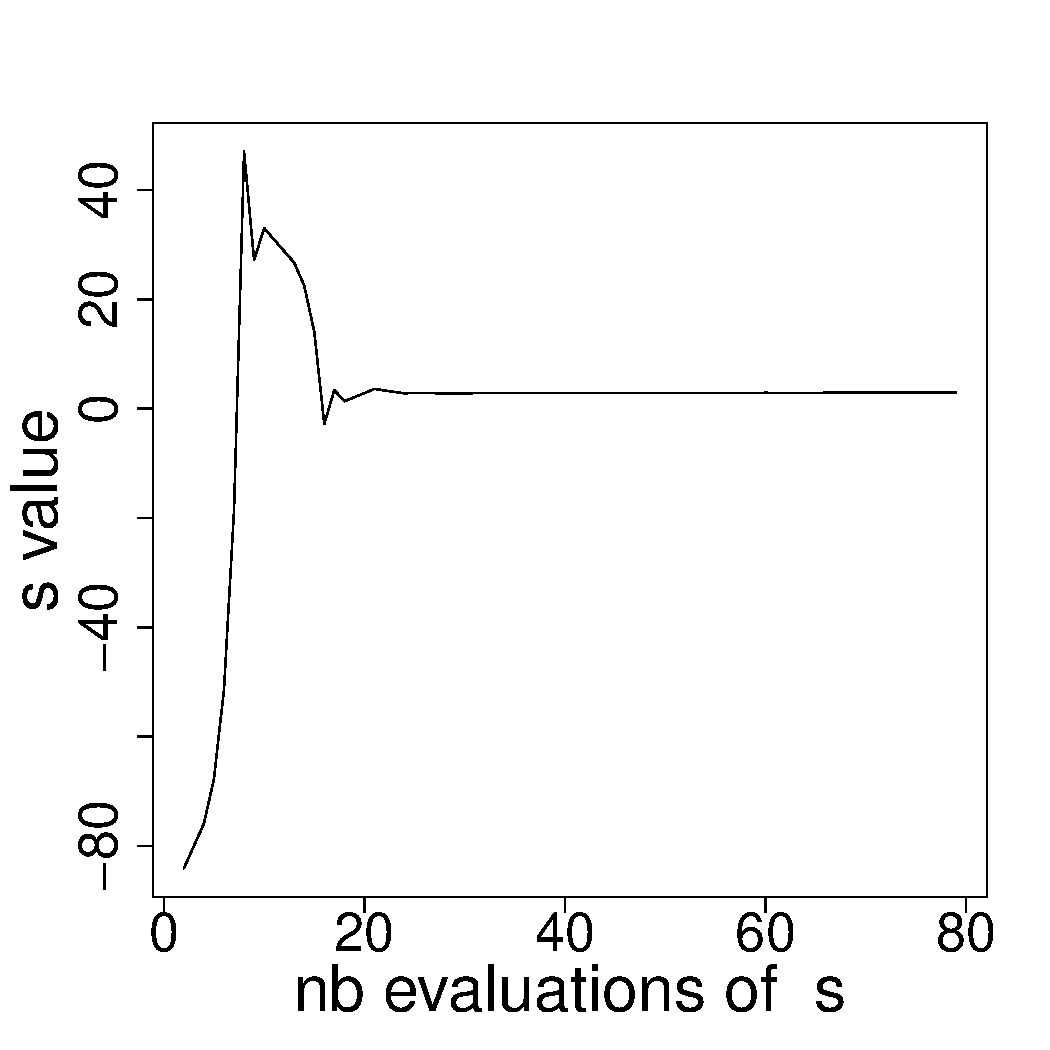
\includegraphics[width=\textwidth]{./R_figs/generated/s_one_run}
		\vspace{-20pt}
		\label{alexandrov_res_one:s}
	\end{minipage}}%
	\subfloat{\begin{minipage}{0.4\textwidth}%
		\centering
		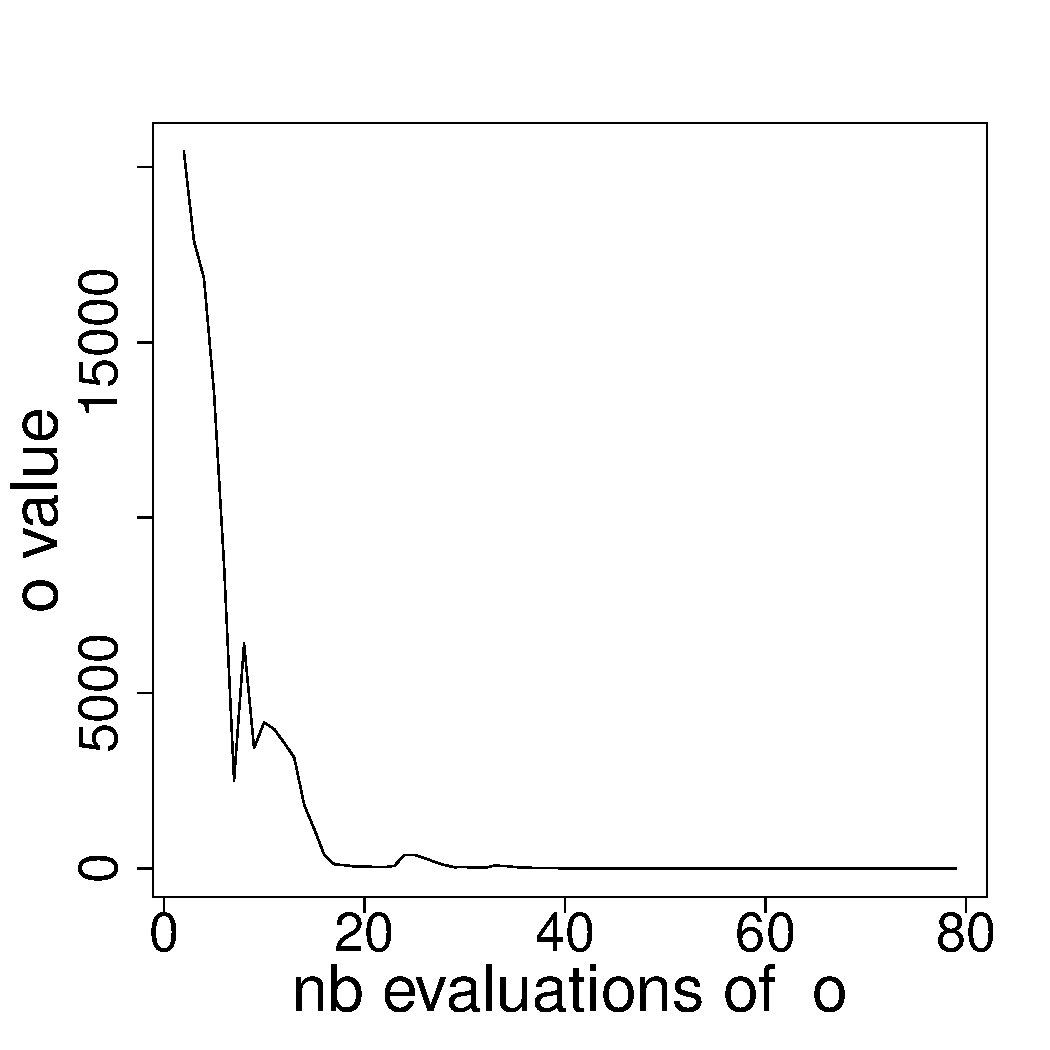
\includegraphics[width=\textwidth]{./R_figs/generated/o_one_run}
		\vspace{-20pt}
		\label{alexandrov_res_one:o}
	\end{minipage}}%
	
	\caption{Alexandrov agents behavior}
	\label{alexandrov_res_one}

\end{figure}

\begin{wrapfigure}{R}{0.4\textwidth}
	\vspace{-50pt}
    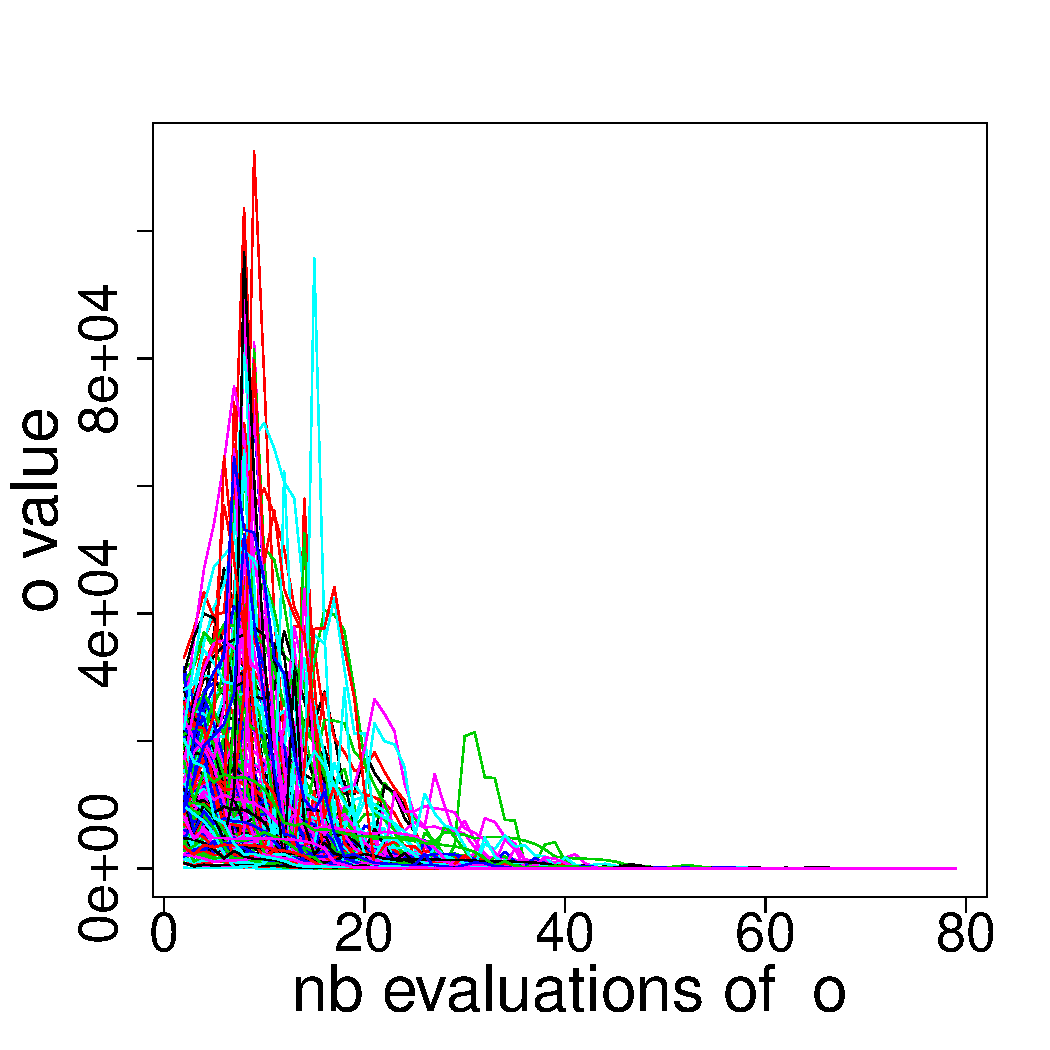
\includegraphics[width=0.4\textwidth]{./R_figs/generated/o}
	\caption{Convergence of the Alexandrov objective for 100 random starting points}
	\label{alexandrov_res}
	\vspace{-25pt}
\end{wrapfigure}

Our first test case is inspired from an academic example taken in literature by Alexandrov and al\cite{alexandrov2002analytical}. This simple example presents some of the commons characteristics of MDO problems, such as interdependent disciplines and multiple criteria. In the original article, the example was used to illustrate some properties of Collaborative Optimization, which we presented earlier, in terms of reformulation. While the paper only gave the structure of the problem, we adapted it with meaningful values and equations.
The mathematical formulation of the problem and the corresponding agent graph can be seen in \figurename \ref{alexandrov}. Interestingly, the NDMO representation is quite similar to the one adopted by the original authors of the problem.

On \figurename \ref{alexandrov_res_one}, the behavior of the \emph{design variables} agents l1, l2 and s, as well the evolution of the objective, can be observed on one instance of the problem with random starting points. On \figurename \ref{alexandrov_res}, we show the evolution of the objective over 100 iterations with  starting points  for each \emph{design variable} randomly drawn over the interval [-100; 100]. We can see how the system converges towards the same optimum despite the wildly different initial conditions.

\subsubsection*{Adaptation to perturbations}
 
On \figurename \ref{alexandrov_res_pert}, we can observe the reaction of the multi-agent system to a perturbation. During the solving of the previous problem, we changed the threshold of the constraint $s + l_1 \leq 1$ to $s + l_1 \leq -4$ (the change is indicated by a dotted line on the charts). The system dynamically adapts to the constraint changed and converges towards a new solution which satisfies the updated constraint.


\begin{figure}[h]
\centering

  \subfloat{\begin{minipage}{0.4\textwidth}%
		\centering
		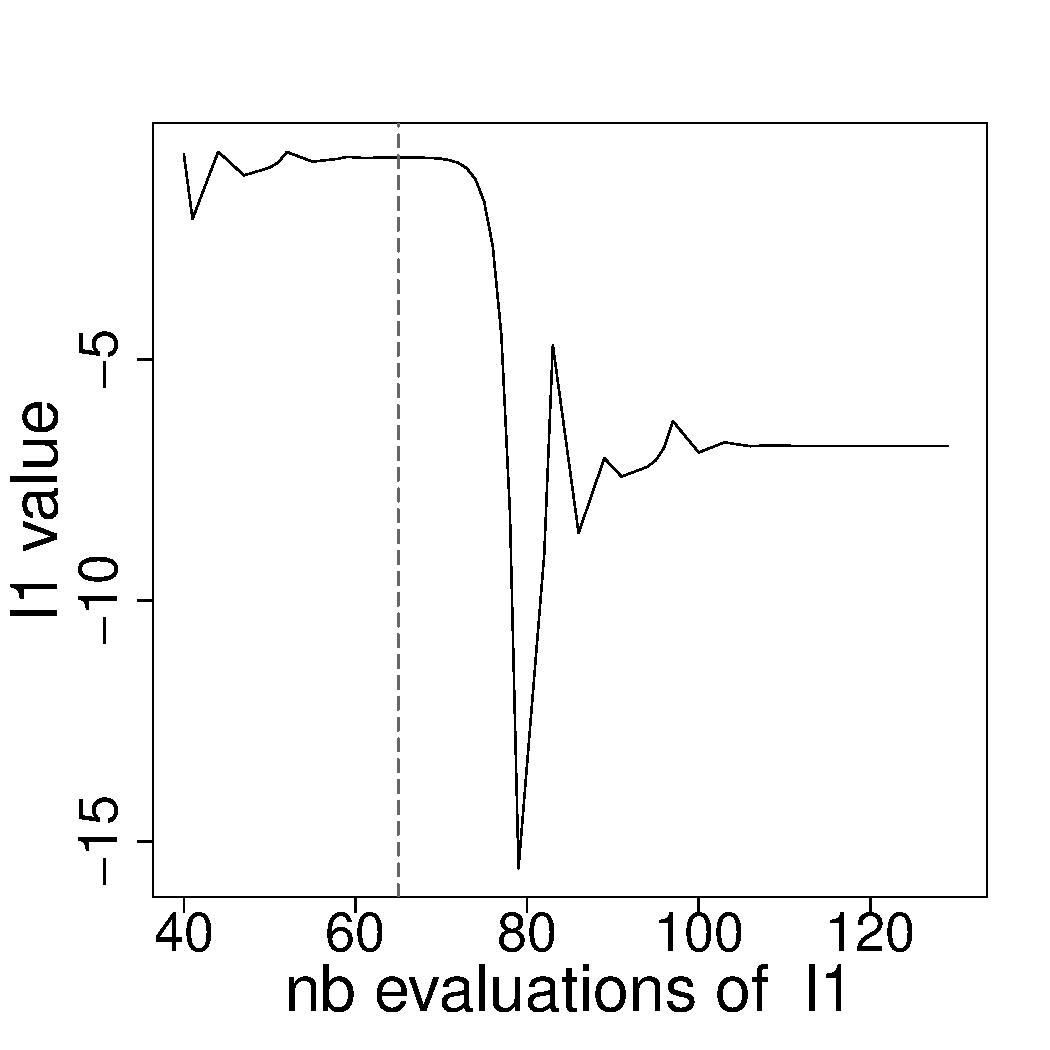
\includegraphics[width=\textwidth]{./R_figs/generated/l1_pertubated}
		\vspace{-20pt}
		\label{alexandrov_res_pert:l1}
	\end{minipage}}%
	\subfloat{\begin{minipage}{0.4\textwidth}%
		\centering
		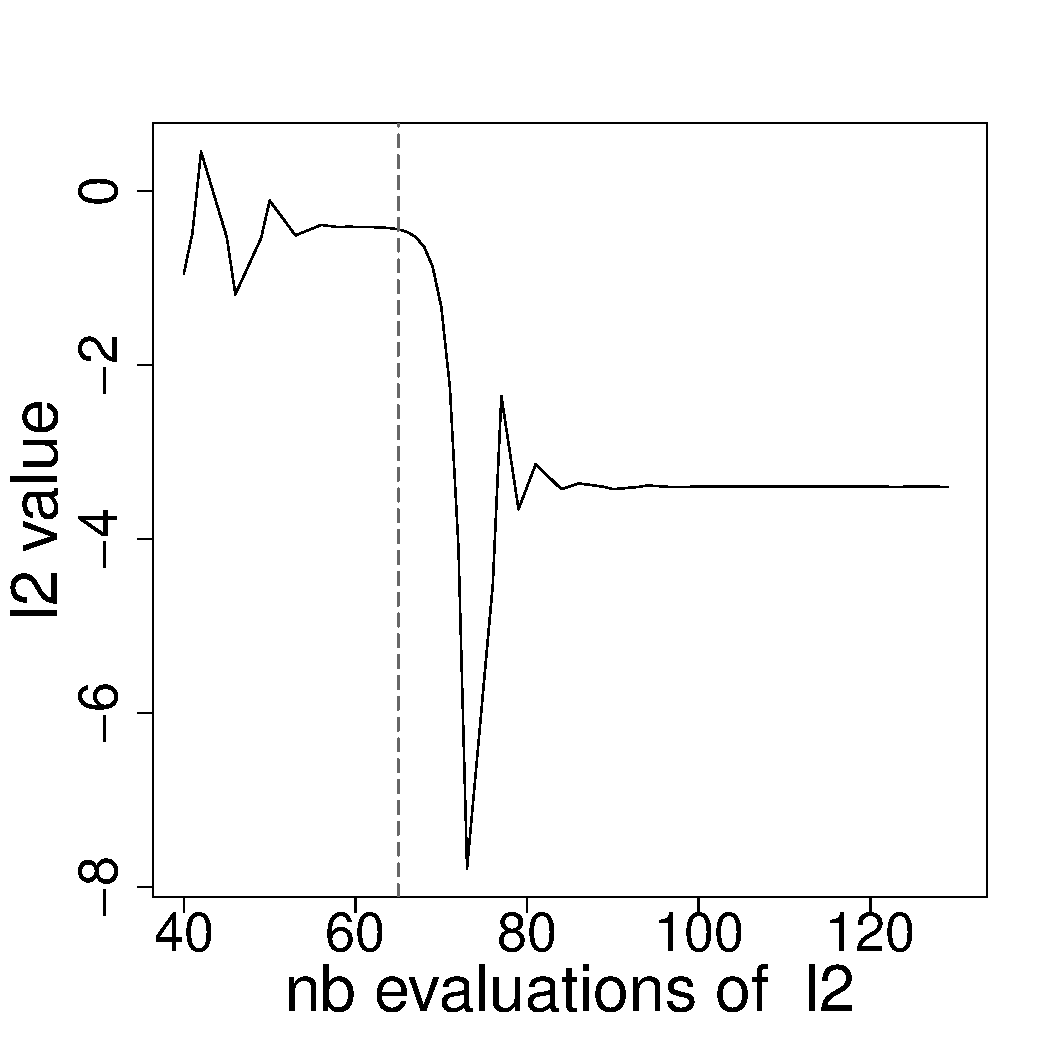
\includegraphics[width=\textwidth]{./R_figs/generated/l2_pertubated}
		\vspace{-20pt}
		\label{alexandrov_res_pert:l2}
	\end{minipage}}
	\vspace{-20pt}
	\\
	\subfloat{\begin{minipage}{0.4\textwidth}%
		\centering
		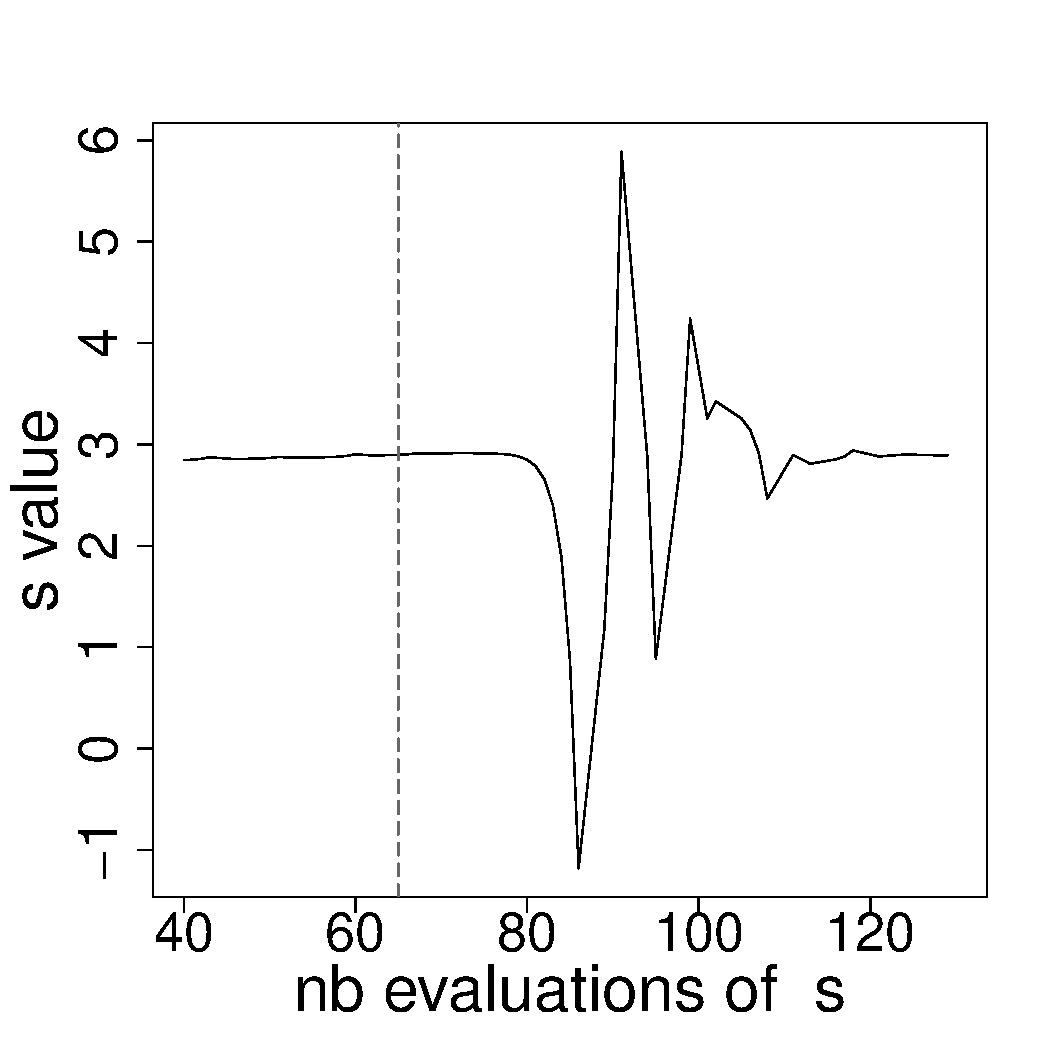
\includegraphics[width=\textwidth]{./R_figs/generated/s_pertubated}
		\vspace{-20pt}
		\label{alexandrov_res_pert:s}
	\end{minipage}}%
	\subfloat{\begin{minipage}{0.4\textwidth}%
		\centering
		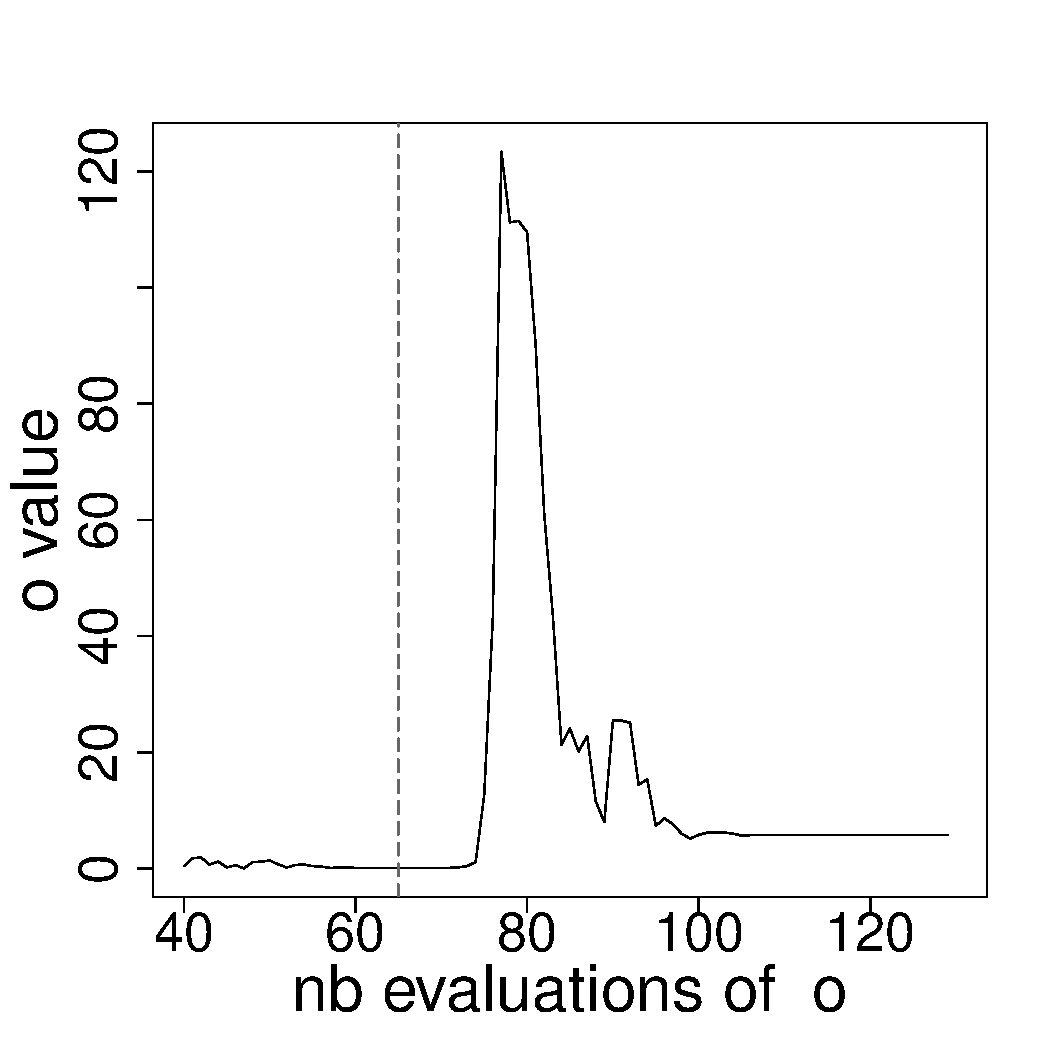
\includegraphics[width=\textwidth]{./R_figs/generated/o_pertubated}
		\vspace{-20pt}
		\label{alexandrov_res_pert:o}
	\end{minipage}}%
	
	\caption{Alexandrov agents behavior with perturbation (constraint change at dotted line)}
	\label{alexandrov_res_pert}

\end{figure}


\subsection{Other Experiments}

We now briefly present results we obtained on two others test cases, the Turbofan problem and Viennet1. For each case, the system was executed 100 times with random starting points for each \emph{design variable}.

\subsubsection{Turbofan Problem}

The turbofan problem we introduced in \figurename \ref{turbofan} is a based on a real-world optimization problem, albeit simplified for demonstration purpose, concerning the conception of a turbofan engine.

As stated before, the problem concerns two \emph{design variables} $pi\_c$ and $bpr$. $pi\_c$ is defined inside the interval [20-40] and $bpr$ inside [2-10]. The model produces three variables $Tdm0$, $s$ and $fr$.
The problem has two objectives, maximizing  $Tdm0$ and minimizing $s$, under the constraint \(s \leq 155\) and \(fr \geq 4\).
The main interest and difficulty of this problem is the existence of two contradictory objectives.
As we can see on \figurename \ref{snecma_res}, the system consistently converges toward the same optimal solution.

\begin{figure}[h]
	\subfloat{\begin{minipage}{0.49\textwidth}%
		\centering
		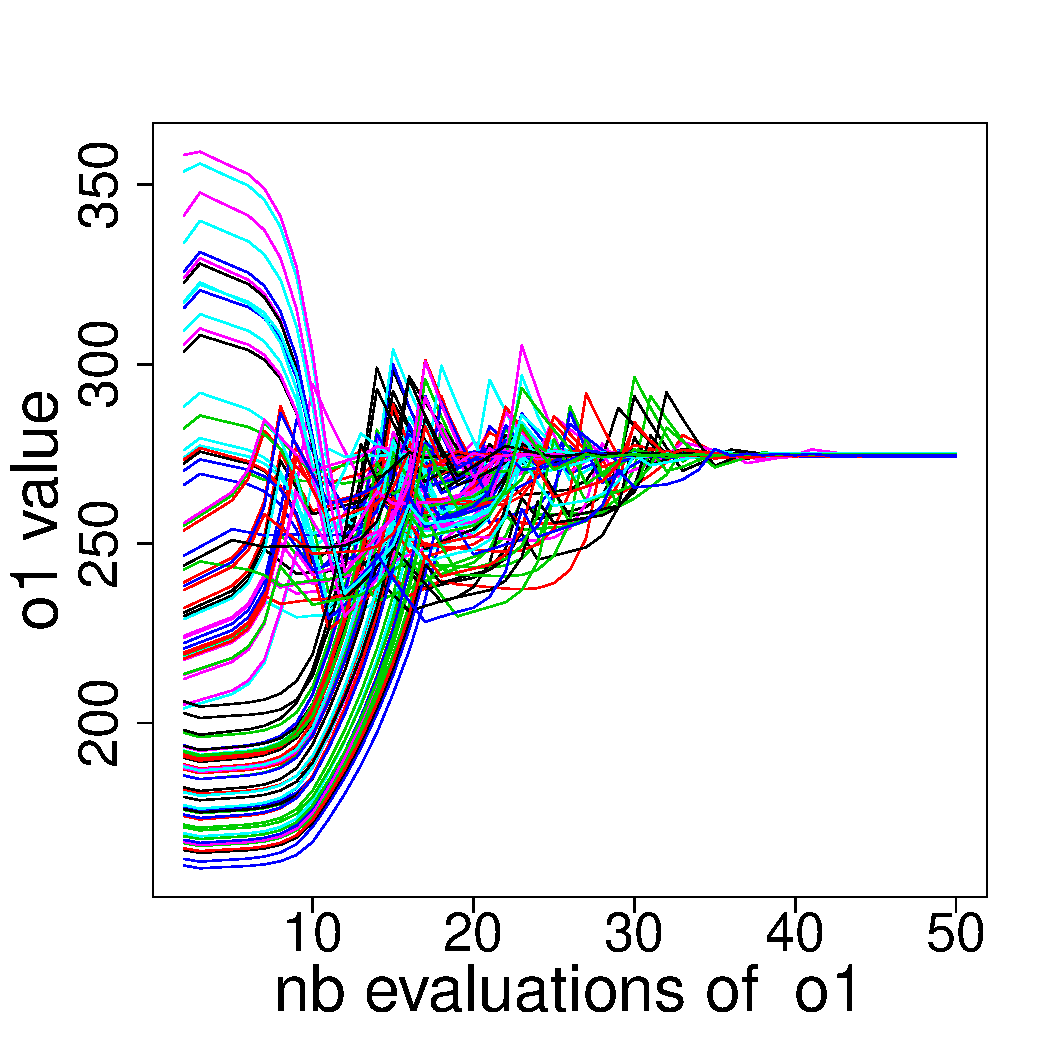
\includegraphics[width = \textwidth]{./R_figs/generated/o1}	
	\end{minipage}}%
	\hfill%for spacing
	\subfloat{\begin{minipage}{0.49\textwidth}%
		\centering
		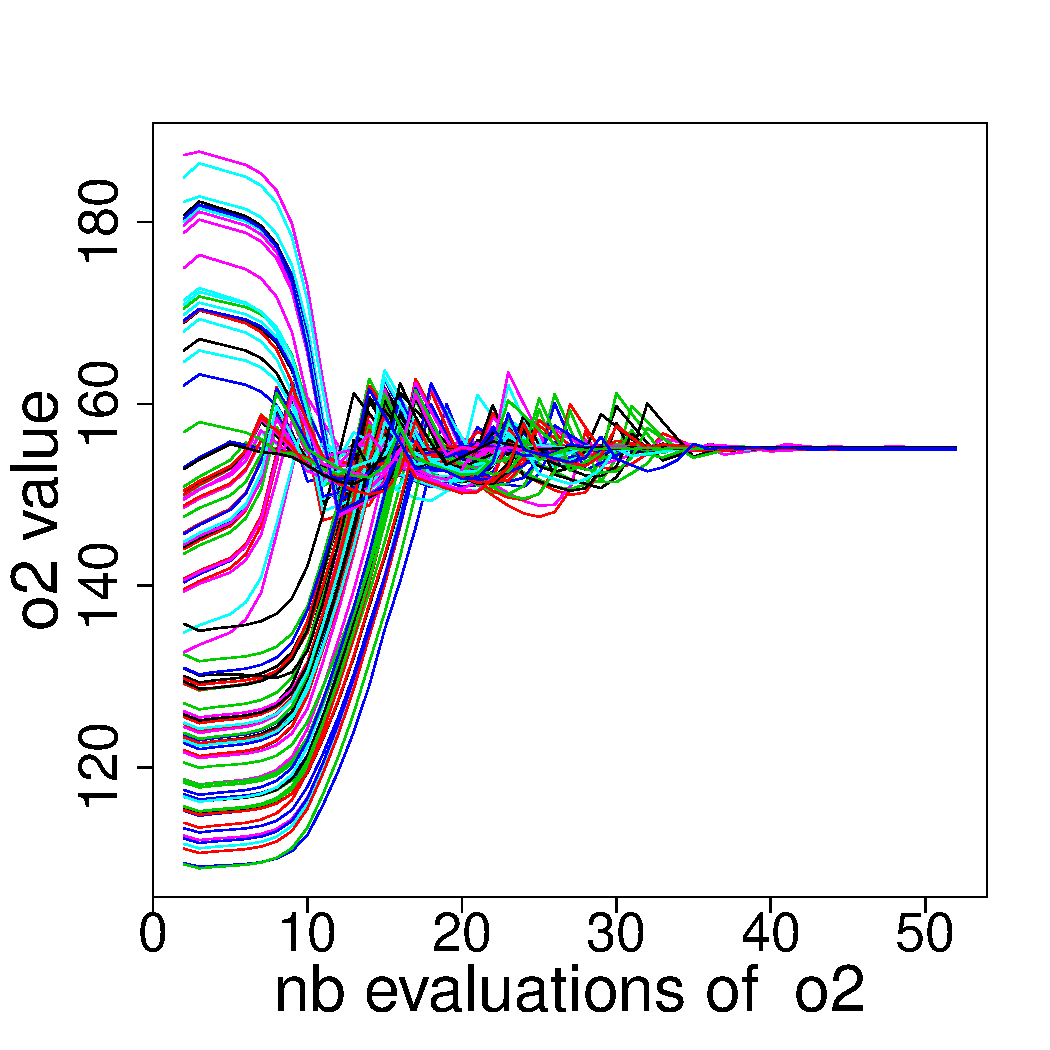
\includegraphics[width = \textwidth]{./R_figs/generated/o2}	
	\end{minipage}}%
	\caption{Convergence of the Turbofan objectives for 100 random starting points}
	\label{snecma_res}
\end{figure}

\subsubsection{Viennet1}

The Viennet1 test case is part of a series of problems proposed in \cite{viennet1996multicriteria} to evaluate multi-criteria optimization techniques. This problem involves three objectives. Its analytical formulation is:


$$\text{Minimize } o1 = x^2 + (y-1)^2 \text{, } o2 = x^2 + (y+1)^2 \text{ and } o3 = (x-1)^2 + y^2 +2\\$$
$$\text{where } x, y \in  [-4;4]
$$

\figurename \ref{viennet_res} illustrates the convergence of the system towards a valid solution.


\begin{figure}[h]

	\subfloat{\begin{minipage}{0.33\textwidth}%
		\centering
		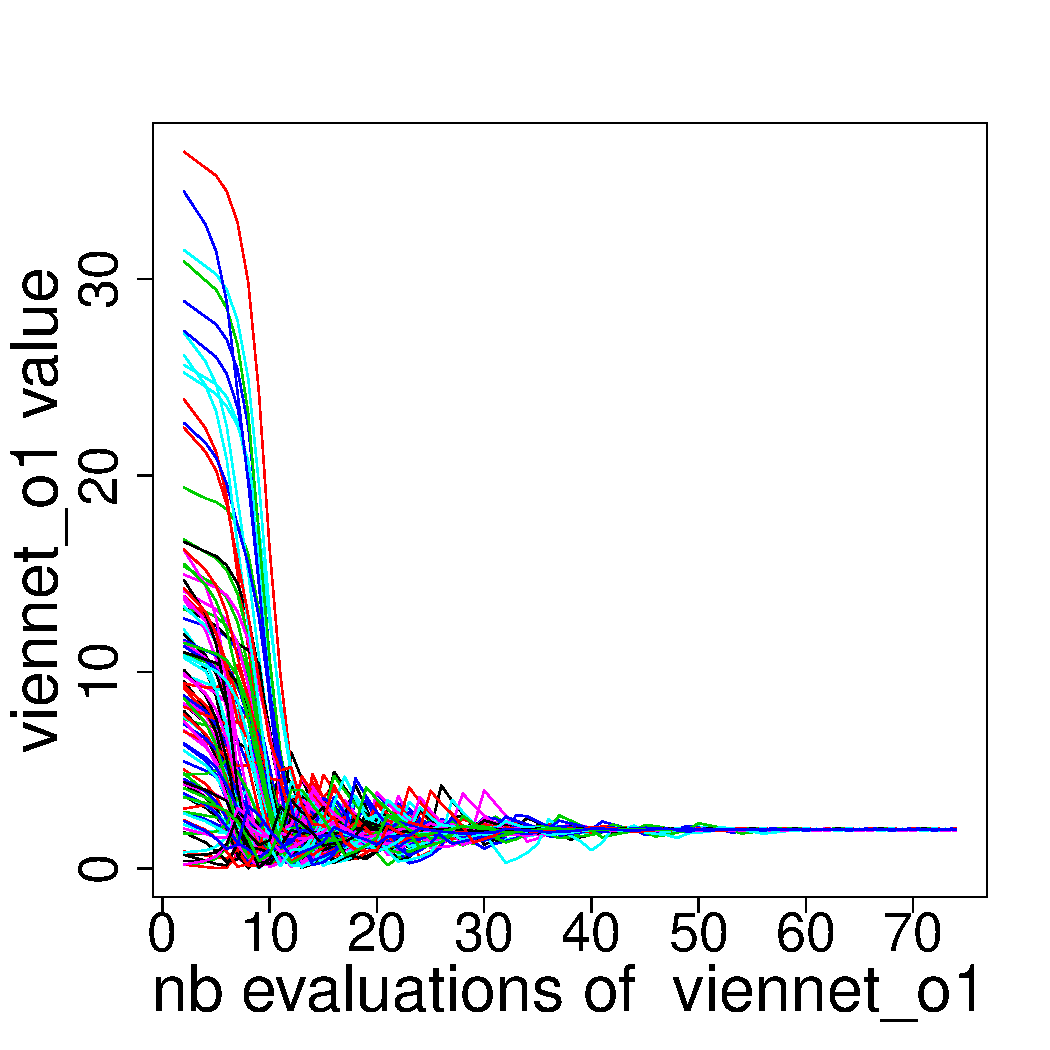
\includegraphics[width = \textwidth]{./R_figs/generated/viennet_o1}	
	\end{minipage}}%
	\hfill%for spacing
	\subfloat{\begin{minipage}{0.33\textwidth}%
		\centering
		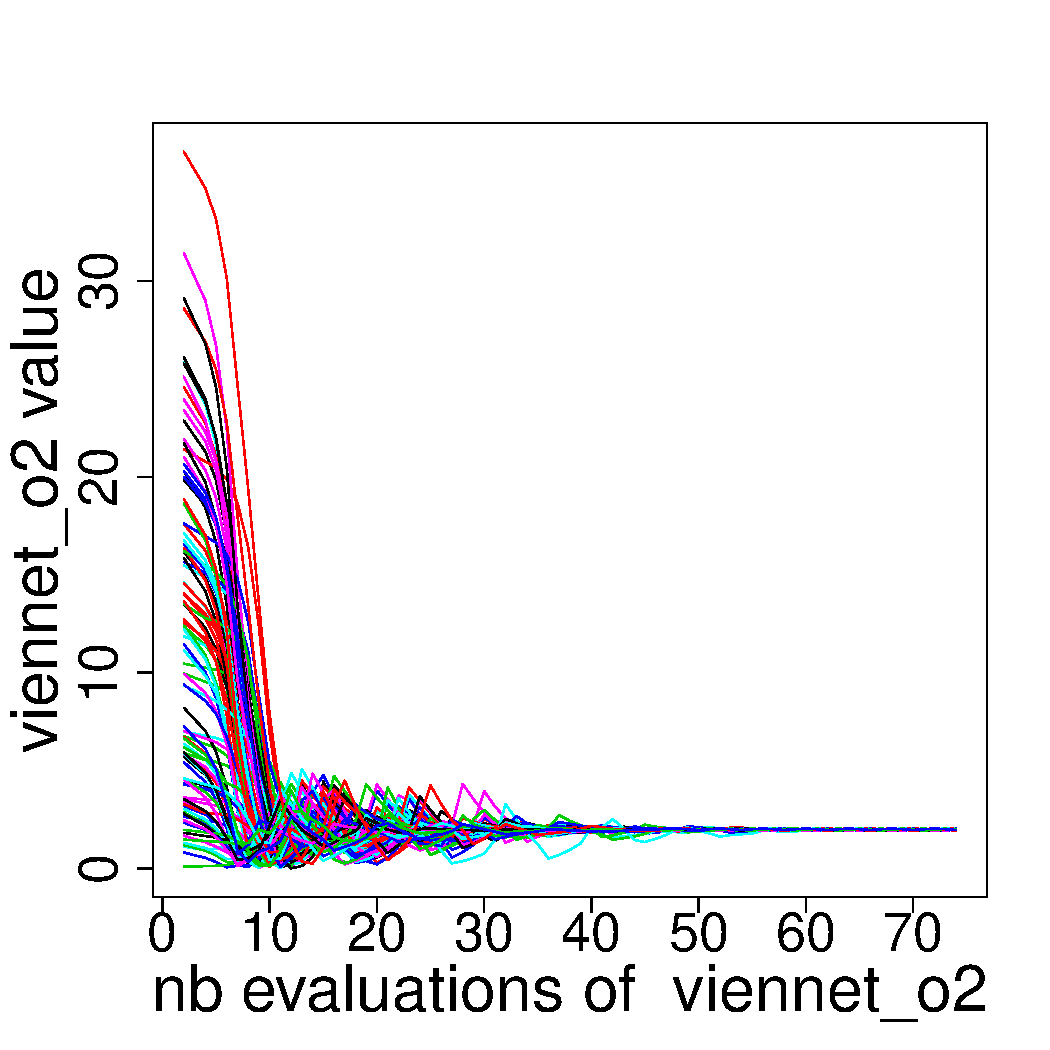
\includegraphics[width = \textwidth]{./R_figs/generated/viennet_o2}	
	\end{minipage}}%
	\hfill%for spacing
	\subfloat{\begin{minipage}{0.33\textwidth}%
		\centering
		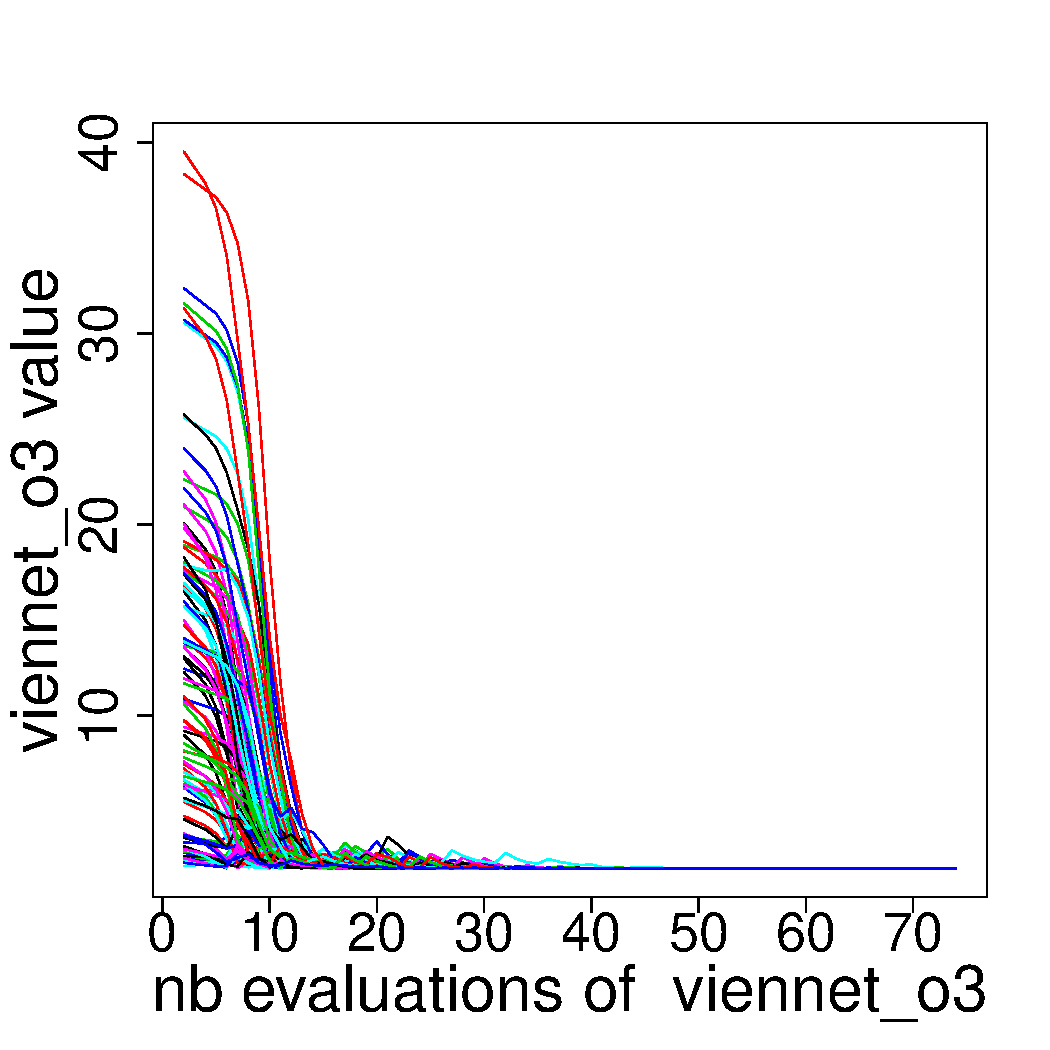
\includegraphics[width = \textwidth]{./R_figs/generated/viennet_o3}	
	\end{minipage}}%
	\caption{Convergence of Viennet1 objectives for 100 random starting points}
	\label{viennet_res}
\end{figure}

\subsubsection{Rosenbrock's valley}

Rosenbrock's valley is non-convex function commonly used to test convergence performances. The results presented here are for the two-dimensional version of the problem with a definition domain of [-5; 5] for each \emph{design variable}.
The analytical formulation of this problem (for two dimensions) is 
$$\text{Minimize } f(x,y) = (1-x)^2 + 100(y - x^2)^2$$

\begin{wrapfigure}{R}{0.5\textwidth}
    \vspace{-50pt}
    \includegraphics[width = 0.5\textwidth]{./R_figs/generated/minimizer}	
    	\vspace{-30pt}
	\caption{Convergence of Rosenbrock objective for 100 random starting points}
	\vspace{-20pt}
\end{wrapfigure}